%@@@@@@@@@@@@@@@@@@@@@@@@@@@@@@@@@@@@@@@@@@@@@@@@@@
\appendix{Appendices}
\label{app:AppendixA}
%@@@@@@@@@@@@@@@@@@@@@@@@@@@@@@@@@@@@@@@@@@@@@@@@@@
%%#################################
%\newpage
%\section{Notation}
%%#################################

%\begin{figure}
%\centering
%\includegraphics[width=1.0\textwidth]{figs/RVQ_CAC_matrix_notation.pdf}
%\caption{RVQ, matrix notation}
%\label{fig:RVQ_CAC_matrix_notation}
%\end{figure}


%########################
\section{Tracking error}
\label{app:Tracking_error_all_datasets}	
\newpage
%########################

\begin{figure}[t]
\centering	
\subfigure[frames 1, 100, 200, 300, 400]{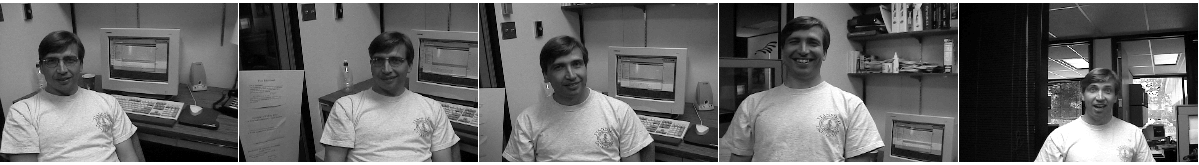
\includegraphics[height=0.1\textheight]{figs/seq_1_Dudek.png}}
\subfigure[iPCA]{\includegraphics[width=0.45\textwidth]{figs/results_errTrk_3_____1___Dudek___________ipca.pdf}}
\subfigure[bPCA]{\includegraphics[width=0.45\textwidth]{figs/results_errTrk_3_____1___Dudek___________bpca.pdf}}
\subfigure[RVQ]{\includegraphics[width=0.45\textwidth]{figs/results_errTrk_3_____1___Dudek___________rvq.pdf}}
\subfigure[TSVQ]{\includegraphics[width=0.45\textwidth]{figs/results_errTrk_3_____1___Dudek___________tsvq.pdf}}		
\caption{Sequence Dudek, tracking error.}										
\label{fig:results_errTrk_3_____1___Dudek}				
\end{figure}
\clearpage



\begin{figure}[t]
\centering	
\subfigure[frames 1, 100, 200, 300, 400]{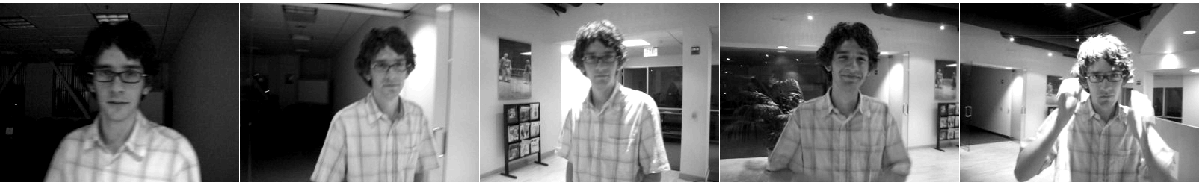
\includegraphics[height=0.1\textheight]{figs/seq_2_davidin300.png}}
\subfigure[iPCA]{\includegraphics[width=0.45\textwidth]{figs/results_errTrk_3_____2___davidin300______ipca.pdf}}
\subfigure[bPCA]{\includegraphics[width=0.45\textwidth]{figs/results_errTrk_3_____2___davidin300______bpca.pdf}}
\subfigure[RVQ]{\includegraphics[width=0.45\textwidth]{figs/results_errTrk_3_____2___davidin300______rvq.pdf}}
\subfigure[TSVQ]{\includegraphics[width=0.45\textwidth]{figs/results_errTrk_3_____2___davidin300______tsvq.pdf}}		
\caption{Sequence davidin300, tracking error.}										
\label{fig:results_errTrk_3_____davidin300_2}				
\end{figure}
\clearpage



\begin{figure}[t]
\centering	
\subfigure[frames 1, 100, 200, 300, 400]{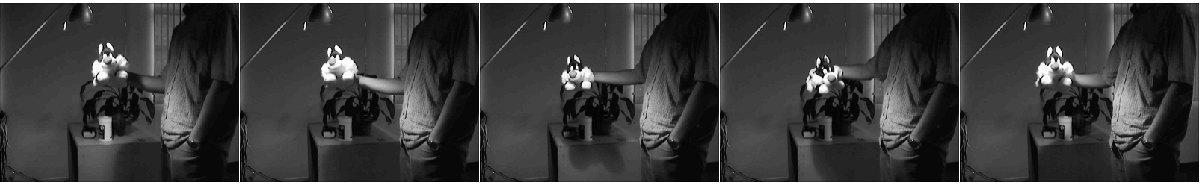
\includegraphics[height=0.1\textheight]{figs/seq_3_sylv.png}}
\subfigure[iPCA]{\includegraphics[width=0.45\textwidth]{figs/results_errTrk_3_____3___sylv____________ipca.pdf}}
\subfigure[bPCA]{\includegraphics[width=0.45\textwidth]{figs/results_errTrk_3_____3___sylv____________bpca.pdf}}
\subfigure[RVQ]{\includegraphics[width=0.45\textwidth]{figs/results_errTrk_3_____3___sylv____________rvq.pdf}}
\subfigure[TSVQ]{\includegraphics[width=0.45\textwidth]{figs/results_errTrk_3_____3___sylv____________tsvq.pdf}}		
\caption{Sequence sylv, tracking error.}										
\label{fig:results_errTrk_3_____sylv_2}				
\end{figure}
\clearpage




%\begin{figure}[t]
%\centering	
%\subfigure[frames 1, 100, 200, 300, 400]{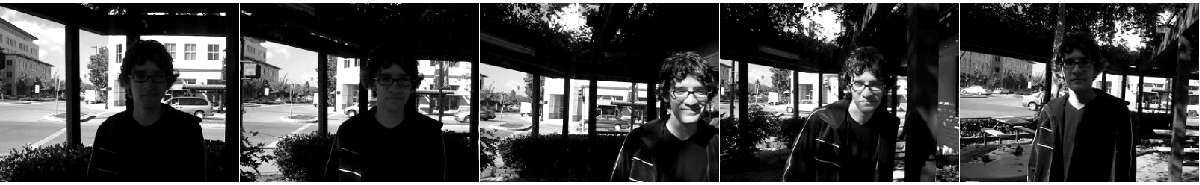
\includegraphics[height=0.1\textheight]{figs/seq_4_trellis70.png}}
%\subfigure[iPCA]{\includegraphics[width=0.45\textwidth]{figs/results_errTrk_3_____4___trellis70_______ipca.pdf}}
%\subfigure[bPCA]{\includegraphics[width=0.45\textwidth]{figs/results_errTrk_3_____4___trellis70_______bpca.pdf}}
%\subfigure[RVQ]{\includegraphics[width=0.45\textwidth]{figs/results_errTrk_3_____4___trellis70_______rvq.pdf}}
%\subfigure[TSVQ]{\includegraphics[width=0.45\textwidth]{figs/results_errTrk_3_____4___trellis70_______tsvq.pdf}}		
%\caption{Sequence trellis70, tracking error.}										
%\label{fig:results_errTrk_3_____trellis70_2}				
%\end{figure}
%\clearpage



\begin{figure}[t]
\centering	
\subfigure[frames 1, 100, 200, 300, 400]{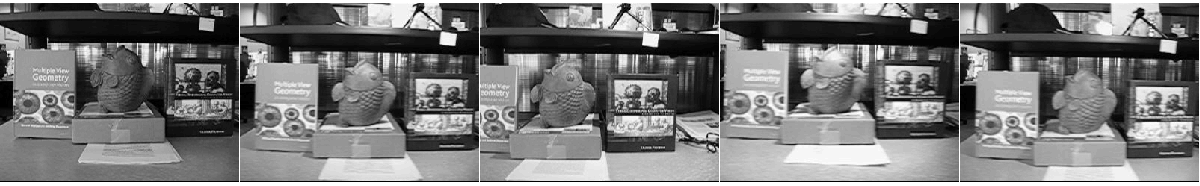
\includegraphics[height=0.1\textheight]{figs/seq_5_fish.png}}
\subfigure[iPCA]{\includegraphics[width=0.45\textwidth]{figs/results_errTrk_3_____5___fish___________ipca.pdf}}
\subfigure[bPCA]{\includegraphics[width=0.45\textwidth]{figs/results_errTrk_3_____5___fish___________bpca.pdf}}
\subfigure[RVQ]{\includegraphics[width=0.45\textwidth]{figs/results_errTrk_3_____5___fish___________rvq.pdf}}
\subfigure[TSVQ]{\includegraphics[width=0.45\textwidth]{figs/results_errTrk_3_____5___fish___________tsvq.pdf}}		
\caption{Sequence fish, tracking error.}										
\label{fig:results_errTrk_3_____fish_2}				
\end{figure}
\clearpage



\begin{figure}[t]
\centering	
\subfigure[frames 1, 100, 200, 300, 400]{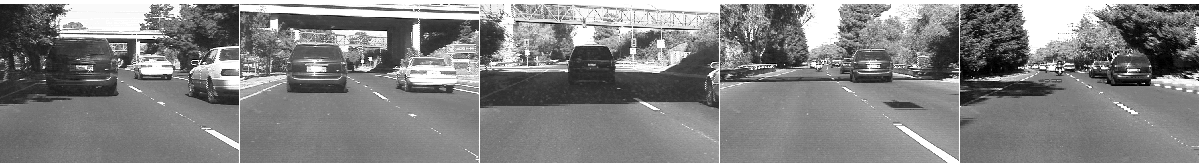
\includegraphics[height=0.1\textheight]{figs/seq_6_car4.png}}
\subfigure[iPCA]{\includegraphics[width=0.45\textwidth]{figs/results_errTrk_3_____6___car4____________ipca.pdf}}
\subfigure[bPCA]{\includegraphics[width=0.45\textwidth]{figs/results_errTrk_3_____6___car4____________bpca.pdf}}
\subfigure[RVQ]{\includegraphics[width=0.45\textwidth]{figs/results_errTrk_3_____6___car4____________rvq.pdf}}
\subfigure[TSVQ]{\includegraphics[width=0.45\textwidth]{figs/results_errTrk_3_____6___car4____________tsvq.pdf}}		
\caption{Sequence car4, tracking error.}										
\label{fig:results_errTrk_3_____car4_2}				
\end{figure}
\clearpage




\begin{figure}[t]
\centering	
\subfigure[frames 1, 100, 200, 300]{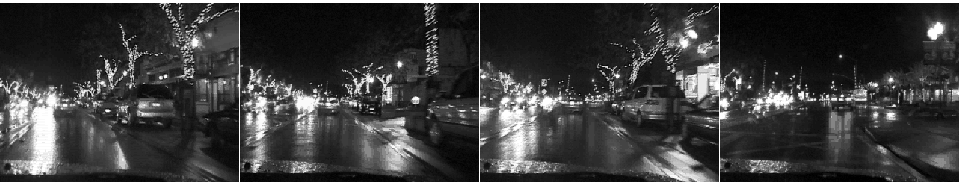
\includegraphics[height=0.1\textheight]{figs/seq_7_car11.png}}
\subfigure[iPCA]{\includegraphics[width=0.45\textwidth]{figs/results_errTrk_3_____7___car11___________ipca.pdf}}
\subfigure[bPCA]{\includegraphics[width=0.45\textwidth]{figs/results_errTrk_3_____7___car11___________bpca.pdf}}
\subfigure[RVQ]{\includegraphics[width=0.45\textwidth]{figs/results_errTrk_3_____7___car11___________rvq.pdf}}
\subfigure[TSVQ]{\includegraphics[width=0.45\textwidth]{figs/results_errTrk_3_____7___car11___________tsvq.pdf}}		
\caption{Sequence car11, tracking error.}										
\label{fig:results_errTrk_3_____car11_2}				
\end{figure}
\clearpage


%########################
\newpage
\section{Tracking, test and training error}
\label{app:RVQ_sw_flowDiagram}	
%########################
The following pages contain training and test error for the 7 datasets used for PCA, RVQ and TSVQ based tracking.

%errTrg and errTst
\begin{figure}[htp]
\centering	
\subfigure[frames 1, 100, 200, 300, 400]{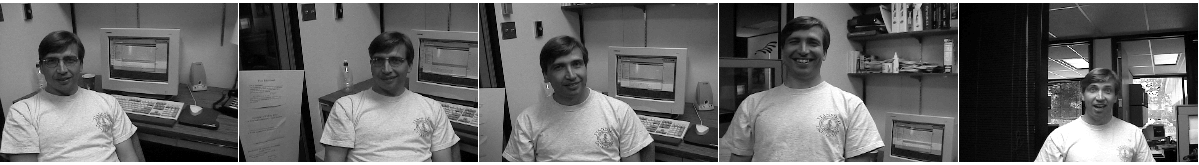
\includegraphics[height=0.1\textheight]{figs/seq_1_Dudek.png}}
\subfigure[iPCA test error]{\includegraphics[width=0.3\textwidth]{figs/results_errTst_5_____1___Dudek___________ipca.pdf}}\\
\subfigure[bPCA training error]{\includegraphics[width=0.3\textwidth]{figs/results_errTrg_4_____1___Dudek___________bpca.pdf}}
\subfigure[bPCA test error]{\includegraphics[width=0.3\textwidth]{figs/results_errTst_5_____1___Dudek___________bpca.pdf}}\\
\subfigure[RVQ training error]{\includegraphics[width=0.3\textwidth]{figs/results_errTrg_4_____1___Dudek___________rvq.pdf}}
\subfigure[RVQ test error]{\includegraphics[width=0.3\textwidth]{figs/results_errTst_5_____1___Dudek___________rvq.pdf}}\\
\subfigure[TSVQ training error]{\includegraphics[width=0.3\textwidth]{figs/results_errTrg_4_____1___Dudek___________tsvq.pdf}}		
\subfigure[TSVQ test error]{\includegraphics[width=0.3\textwidth]{figs/results_errTst_5_____1___Dudek___________tsvq.pdf}}
\caption{Sequence Dudek, training and test error.}										
\label{fig:results_errTrg_4_____Dudek}				
\end{figure}
\clearpage



\begin{figure}[htp]
\centering	
\subfigure[frames 1, 100, 200, 300, 400]{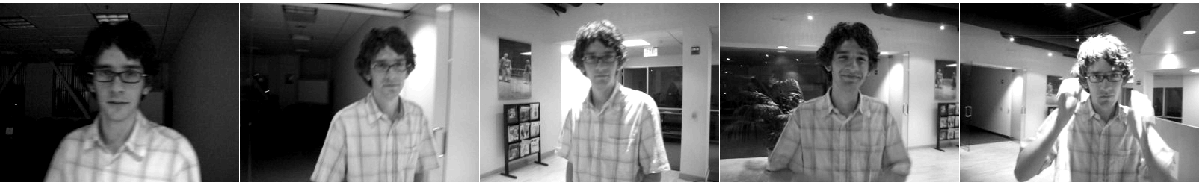
\includegraphics[height=0.1\textheight]{figs/seq_2_davidin300.png}}
\subfigure[iPCA test error]{\includegraphics[width=0.3\textwidth]{figs/results_errTst_5_____2___davidin300______ipca.pdf}}\\
\subfigure[bPCA training error]{\includegraphics[width=0.3\textwidth]{figs/results_errTrg_4_____2___davidin300______bpca.pdf}}
\subfigure[bPCA test error]{\includegraphics[width=0.3\textwidth]{figs/results_errTst_5_____2___davidin300______bpca.pdf}}\\
\subfigure[RVQ training error]{\includegraphics[width=0.3\textwidth]{figs/results_errTrg_4_____2___davidin300______rvq.pdf}}
\subfigure[RVQ test error]{\includegraphics[width=0.3\textwidth]{figs/results_errTst_5_____2___davidin300______rvq.pdf}}\\
\subfigure[TSVQ training error]{\includegraphics[width=0.3\textwidth]{figs/results_errTrg_4_____2___davidin300______tsvq.pdf}}		
\subfigure[TSVQ test error]{\includegraphics[width=0.3\textwidth]{figs/results_errTst_5_____2___davidin300______tsvq.pdf}}		
\caption{Sequence davidin300, training and test error.}										
\label{fig:results_errTrg_4_____davidin300}				
\end{figure}
\clearpage



\begin{figure}[htp]
\centering	
\subfigure[frames 1, 100, 200, 300, 400]{\includegraphics[height=0.1\textheight]{figs/seq_3_sylv.png}}
\subfigure[iPCA test error]{\includegraphics[width=0.3\textwidth]{figs/results_errTst_5_____3___sylv____________ipca.pdf}}\\
\subfigure[bPCA training error]{\includegraphics[width=0.3\textwidth]{figs/results_errTrg_4_____3___sylv____________bpca.pdf}}
\subfigure[bPCA test error]{\includegraphics[width=0.3\textwidth]{figs/results_errTst_5_____3___sylv____________bpca.pdf}}\\
\subfigure[RVQ training error]{\includegraphics[width=0.3\textwidth]{figs/results_errTrg_4_____3___sylv____________rvq.pdf}}
\subfigure[RVQ test error]{\includegraphics[width=0.3\textwidth]{figs/results_errTst_5_____3___sylv____________rvq.pdf}}\\
\subfigure[TSVQ training error]{\includegraphics[width=0.3\textwidth]{figs/results_errTrg_4_____3___sylv____________tsvq.pdf}}		
\subfigure[TSVQ test error]{\includegraphics[width=0.3\textwidth]{figs/results_errTst_5_____3___sylv____________tsvq.pdf}}		
\caption{Sequence sylv, training and test error.}										
\label{fig:results_errTrg_4_____sylv}				
\end{figure}
\clearpage



%\begin{figure}[htp]
%\centering	
%\subfigure[frames 1, 100, 200, 300, 400]{\includegraphics[height=0.1\textheight]{figs/seq_4_trellis70.png}}
%\subfigure[iPCA test error]{\includegraphics[width=0.3\textwidth]{figs/results_errTst_5_____4___trellis70_______ipca.pdf}}\\
%\subfigure[bPCA training error]{\includegraphics[width=0.3\textwidth]{figs/results_errTrg_4_____4___trellis70_______bpca.pdf}}
%\subfigure[bPCA test error]{\includegraphics[width=0.3\textwidth]{figs/results_errTst_5_____4___trellis70_______bpca.pdf}}\\
%\subfigure[RVQ training error]{\includegraphics[width=0.3\textwidth]{figs/results_errTrg_4_____4___trellis70_______rvq.pdf}}
%\subfigure[RVQ test error]{\includegraphics[width=0.3\textwidth]{figs/results_errTst_5_____4___trellis70_______rvq.pdf}}\\
%\subfigure[TSVQ training error]{\includegraphics[width=0.3\textwidth]{figs/results_errTrg_4_____4___trellis70_______tsvq.pdf}}		
%\subfigure[TSVQ test error]{\includegraphics[width=0.3\textwidth]{figs/results_errTst_5_____4___trellis70_______tsvq.pdf}}		
%\caption{Sequence trellis70, training and test error.}										
%\label{fig:results_errTrg_4_____trellis70}				
%\end{figure}
%\clearpage



\begin{figure}[htp]
\centering	
\subfigure[frames 1, 100, 200, 300, 400]{\includegraphics[height=0.1\textheight]{figs/seq_5_fish.png}}
\subfigure[iPCA test error]{\includegraphics[width=0.3\textwidth]{figs/results_errTst_5_____5___fish___________ipca.pdf}}\\
\subfigure[bPCA training error]{\includegraphics[width=0.3\textwidth]{figs/results_errTrg_4_____5___fish___________bpca.pdf}}
\subfigure[bPCA test error]{\includegraphics[width=0.3\textwidth]{figs/results_errTst_5_____5___fish___________bpca.pdf}}\\
\subfigure[RVQ training error]{\includegraphics[width=0.3\textwidth]{figs/results_errTrg_4_____5___fish___________rvq.pdf}}
\subfigure[RVQ test error]{\includegraphics[width=0.3\textwidth]{figs/results_errTst_5_____5___fish___________rvq.pdf}}\\
\subfigure[TSVQ training error]{\includegraphics[width=0.3\textwidth]{figs/results_errTrg_4_____5___fish___________tsvq.pdf}}		
\subfigure[TSVQ test error]{\includegraphics[width=0.3\textwidth]{figs/results_errTst_5_____5___fish___________tsvq.pdf}}		
\caption{Sequence fish, training and test error.}										
\label{fig:results_errTrg_4_____fish}				
\end{figure}
\clearpage



\begin{figure}[htp]
\centering	
\subfigure[frames 1, 100, 200, 300, 400]{\includegraphics[height=0.1\textheight]{figs/seq_6_car4.png}}
\subfigure[iPCA training error]{\includegraphics[width=0.3\textwidth]{figs/results_errTst_5_____6___car4____________ipca.pdf}}\\
\subfigure[bPCA training error]{\includegraphics[width=0.3\textwidth]{figs/results_errTrg_4_____6___car4____________bpca.pdf}}
\subfigure[bPCA test error]{\includegraphics[width=0.3\textwidth]{figs/results_errTst_5_____6___car4____________bpca.pdf}}\\
\subfigure[RVQ training error]{\includegraphics[width=0.3\textwidth]{figs/results_errTrg_4_____6___car4____________rvq.pdf}}
\subfigure[RVQ test error]{\includegraphics[width=0.3\textwidth]{figs/results_errTst_5_____6___car4____________rvq.pdf}}\\
\subfigure[TSVQ training error]{\includegraphics[width=0.3\textwidth]{figs/results_errTrg_4_____6___car4____________tsvq.pdf}}		
\subfigure[TSVQ test error]{\includegraphics[width=0.3\textwidth]{figs/results_errTst_5_____6___car4____________tsvq.pdf}}		
\caption{Sequence car4, training and test error.}										
\label{fig:results_errTrg_4_____car4}				
\end{figure}
\clearpage




\begin{figure}[htp]
\centering	
\subfigure[frames 1, 100, 200, 300]{\includegraphics[height=0.1\textheight]{figs/seq_7_car11.png}}
\subfigure[iPCA test error]{\includegraphics[width=0.3\textwidth]{figs/results_errTst_5_____7___car11___________ipca.pdf}}\\
\subfigure[bPCA training error]{\includegraphics[width=0.3\textwidth]{figs/results_errTrg_4_____7___car11___________bpca.pdf}}
\subfigure[bPCA test error]{\includegraphics[width=0.3\textwidth]{figs/results_errTst_5_____7___car11___________bpca.pdf}}\\
\subfigure[RVQ training error]{\includegraphics[width=0.3\textwidth]{figs/results_errTrg_4_____7___car11___________rvq.pdf}}
\subfigure[RVQ test error]{\includegraphics[width=0.3\textwidth]{figs/results_errTst_5_____7___car11___________rvq.pdf}}\\
\subfigure[TSVQ training error]{\includegraphics[width=0.3\textwidth]{figs/results_errTrg_4_____7___car11___________tsvq.pdf}}		
\subfigure[TSVQ test error]{\includegraphics[width=0.3\textwidth]{figs/results_errTst_5_____7___car11___________tsvq.pdf}}		
\caption{Sequence car11, training and test error.}										
\label{fig:results_errTrg_4_____car11}				
\end{figure}
\clearpage

%%########################
%\newpage
%\section{RVQ software flow diagram}
%\label{app:RVQ_sw_flowDiagram}	
%%########################
%
%\begin{figure}[htp]
%	\centering	
%	\subfigure[RVQ training]
%	{
%		\includegraphics[width=1.0\textwidth]{figs/RVQ_software_training.pdf}
%		\label{fig:RVQ_software_training}	
%	}
%	\subfigure[RVQ testing]
%	{
%		\includegraphics[width=0.8\textwidth]{figs/RVQ_software_testing.pdf}
%		\label{fig:RVQ_software_testing}	
%	}		
%	\caption{RVQ training and testing, software flow}
%	\label{fig:RVQ_testing}	
%\end{figure}


%%#################################
%\newpage
%\section{Variables}
%%#################################

%\begin{table}[hp]
%\center
%\begin{tabular}{|c|c|c|c|c|}\hline 
%	 					&{\color{red}iPCA} 		&{\color{red}bPCA} 	&{\color{red}TSVQ} 	&{\color{red}RVQ}	\\\hline 
%training parameters 	&- 							&-						&T						&T, S					\\\hline\hline
%training output 		&$U, S, V$, mean 	 		&$U, S, V$, mean 		&codebook 			&codebook 			\\\hline 
%" 						&avg. reconstruction snr 	&same 					&same					&same					\\\hline
%"  						&avg. reconstruction rmse &same					&same					&same					\\\hline\hline
%testing parameters 	&$N_{eig}$ 				&$N_{eig}$			&-						&-						\\\hline\hline
%testing output 			&reconstructed signal 		&same					&same					&same					\\\hline
%" 						&error signal 				&same					&same					&same					\\\hline
%" 						&reconstruction snr 		&same 					&same					&same					\\\hline
%" 						&reconstruction rmse 		&same					&same					&same					\\\hline
%\end{tabular}
%\caption{Training and testing variables, $U, S, V$ are outputs of the SVD operation, $N_{eig}$ is the number of eigenvectors to retain for PCA, $T$ and $S$ are the number of stages and number of codevectors per stage respectively for RVQ, $T$ is the depth for TSVQ (assumed to be binary here)}
%\end{table}


%%########################
%\newpage
%\section{Source code}
%\label{App:source_code}	
%%########################

